\documentclass[12pt, notitlepage, final]{article} 

\newcommand{\name}{Vince Coghlan}

%\usepackage[dvips]{graphics,color}
\usepackage{amsfonts}
\usepackage{amssymb}
\usepackage{amsmath}
\usepackage{latexsym}
\usepackage{enumerate}
\usepackage{amsthm}
\usepackage{nccmath}
\usepackage{setspace}
\usepackage[pdftex]{graphicx}
\usepackage{epstopdf}
\usepackage[siunitx]{circuitikz}
\usepackage{tikz}
\usepackage{float}
\usepackage{cancel} 
\usepackage{setspace}
\usepackage{overpic}
\usepackage{mathtools}
\usepackage{listings}
\usepackage{color}
\usepackage{qtree}
%\usepackage{gensymb}

\usetikzlibrary{calc}
\usetikzlibrary{matrix}
\usetikzlibrary{positioning}

\numberwithin{equation}{section}
\DeclareRobustCommand{\beginProtected}[1]{\begin{#1}}
\DeclareRobustCommand{\endProtected}[1]{\end{#1}}
\newcommand{\dbr}[1]{d_{\mbox{#1BR}}}
\newtheorem{lemma}{Lemma}
\newtheorem*{corollary}{Corollary}
\newtheorem{theorem}{Theorem}
\newtheorem{proposition}{Proposition}
\theoremstyle{definition}
\newtheorem{define}{Definition}
\newcommand{\column}[2]{
\left( \begin{array}{ccc}
#1 \\
#2
\end{array} \right)}

\newdimen\digitwidth
\settowidth\digitwidth{0}
\def~{\hspace{\digitwidth}}

\setlength{\parskip}{1pc}
\setlength{\parindent}{0pt}
\setlength{\topmargin}{-3pc}
\setlength{\textheight}{9.0in}
\setlength{\oddsidemargin}{0pc}
\setlength{\evensidemargin}{0pc}
\setlength{\textwidth}{6.5in}
\newcommand{\answer}[1]{\newpage\noindent\framebox{\vbox{{\bf ECEN 5018 Spring 2014} 
\hfill {\bf \name} \vspace{-1cm}
\begin{center}{Homework \#7}\end{center} } }\bigskip }

\DeclareMathOperator*{\argmin}{arg\,min}

%absolute value code
\DeclarePairedDelimiter\abs{\lvert}{\rvert}%
\DeclarePairedDelimiter\norm{\lVert}{\rVert}
\makeatletter
\let\oldabs\abs
\def\abs{\@ifstar{\oldabs}{\oldabs*}}
%
\let\oldnorm\norm
\def\norm{\@ifstar{\oldnorm}{\oldnorm*}}
\makeatother

\def\dbar{{\mathchar'26\mkern-12mu d}}
\def \Frac{\displaystyle\frac}
\def \Sum{\displaystyle\sum}
\def \Int{\displaystyle\int}
\def \Prod{\displaystyle\prod}
%\def \P[x]{\Frac{\partial}{\partial x}}
%\def \D[x]{\Frac{d}{dx}}
\newcommand{\PD}[2]{\frac{\partial#1}{\partial#2}}
\newcommand{\PF}[1]{\frac{\partial}{\partial#1}}
\newcommand{\DD}[2]{\frac{d#1}{d#2}}
\newcommand{\DF}[1]{\frac{d}{d#1}}
\newcommand{\fix}[2]{\left(#1\right)_#2}
\newcommand{\ket}[1]{|#1\rangle}
\newcommand{\bra}[1]{\langle#1|}
\newcommand{\braket}[2]{\langle #1 | #2 \rangle}
\newcommand{\bopk}[3]{\langle #1 | #2 | #3 \rangle}
\newcommand{\Choose}[2]{\displaystyle {#1 \choose #2}}
\newcommand{\proj}[1]{\ket{#1}\bra{#1}}
\def\del{\vec{\nabla}}
\newcommand{\avg}[1]{\langle#1\rangle}
\newcommand{\piecewise}[4]{\left\{\beginProtected{array}{rl}#1&:#2\\#3&:#4\endProtected{array}\right.}
\newcommand{\systeme}[2]{\left\{\beginProtected{array}{rl}#1\\#2\endProtected{array}\right.}
\def \KE{K\!E}
\def\Godel{G$\ddot{\mbox{o}}$del}

%\onehalfspacing

\begin{document}

\answer{}

\textbf{1)} Consider the following multiagent system (vehicle target assignment problem) with the
following elements:
\begin{itemize}
  \item{Set of vehicles: $\mathcal{V}=\{1,2,3\}$}
  \item{Vehicle detection probability $p_1$, $p_2$, $p_3 \in [0,1]$}
  \item{Set of targets $\mathcal{T}=\{x,y\}$}
  \item{Set of possible assignments for each vehicle: $\mathcal{A}_i=\{x,y\}$, i.e., each vehicle can
    select only on of the two targets}
  \item{Target specific welfare functions: for any set of vehicles $S \subseteq \mathcal{V}$}
  \[
    W_x(S) = v_x\left[1-\prod_{j\in S}(1-p_j)\right]
  \]
  \[
    W_y(S) = v_y\left[1-\prod_{j\in S}(1-p_j)\right]
  \]
  \item{Global objective: Maximize total welfare}
  \[
    W(a) = W_x(\{a\}_x)+W_y(\{a\}_y)
  \]
  where $\{a\}_x = \{i\in\mathcal{V}:t\in a_x\}$.
\end{itemize}

\textbf{Part \#1:} Model the above multiagent system as a game with player set $\mathcal{V}$ and the
wonderful life utility.

\begin{enumerate}[(a)]
  \item{What is the payoff matrix?}\\
    We can find the utility:
    \[
      U_i(a)=\sum_{r\in a_i}(W_r(\{a\}_r)-W_r(\{a\}_r\backslash \{i\}))
    \]

    For example, if player 1 goes to x, and players two and three are not there:
    \[
      U_1(x) = v_x\left[1-\prod_{j\in S}(1-p_1)\right] - 1 = v_xp_1 - 1
    \]
    If player 2 is there:
    \[
      U_1(x) = v_x\left[1-(1-p_2)(1-p_1)\right] - v_x\left[1-(1-p_2)\right]
    \]
    If player 2 and 3 are there:
    \[
      U_1(x) = v_x\left[1-(1-p_3)(1-p_2)(1-p_1)\right] - v_x\left[1-(1-p_2)(1-p_3)\right]
    \]
    Whereas at this specific point player 2 would see:
    \[
      U_2(x) = v_x\left[1-(1-p_3)(1-p_2)(1-p_1)\right] - v_x\left[1-(1-p_3)(1-p_1)\right]
    \]
    This is way too long to fit in a payoff matrix, so ill save writing down the payoff matrix
    until part (c).

  \item{Is the game a potential game? If so, what is the potential function?}\\
    Yes it is a potential game, with a potential function W:
    \[
      \Phi = W_x(\{a\}_x) + W_y(\{a\}_y)
    \]
  \item{From this point on, i.e., all future questions in Part \#1, set $v_x=2$, $v_y=1$, $p_1=1$,
    $p_2 = 1/2$, and $p_3 = 1/4$.  What is the payoff matrix for this specific setting?}\\
    The payoff matrix:
  \begin{center}
  \begin{tabular}{r |c|c|}
    \multicolumn{1}{r}{}
    & \multicolumn{1}{c}{$x$}
    & \multicolumn{1}{c}{$y$}\\
    \cline{2-3}
    $x$ & 3/4, 0, 0 & 3/2, 1/2, 0 \\
    \cline{2-3}
    $y$ & 1, 3/4, 1/4 & 1/2, 0, 1/2 \\
    \cline{2-3}
  \end{tabular}
  \begin{tabular}{r |c|c|}
    \multicolumn{1}{r}{}
    & \multicolumn{1}{c}{$x$}
    & \multicolumn{1}{c}{$y$}\\
    \cline{2-3}
    $x$ & 1, 0, 1/4 & 2, 3/8, 1/8 \\
    \cline{2-3}
    $y$ & 3/4, 1, 0 & 1, 0, 0 \\
    \cline{2-3}
  \end{tabular}\\
  \vspace{2mm}
  \hspace{6mm}$x$\hspace{5.4cm}$y$\\
  \end{center}

  \item{What is the better reply graph?}

  \begin{figure}[H]
  \begin{center}
  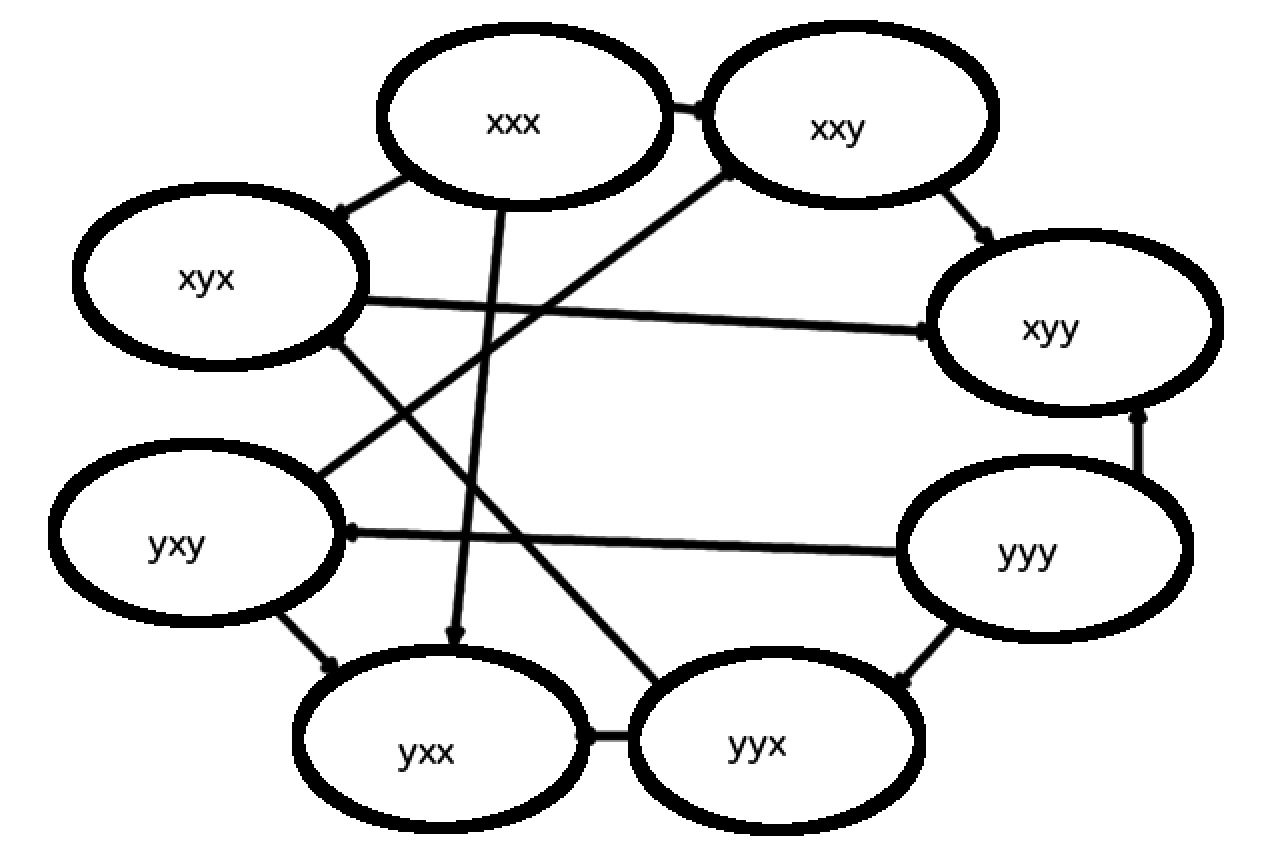
\includegraphics[width=10cm]{f1}
  \end{center}
  \end{figure}

  \item{What are the N.E.?}
  $yxx$ and $xyy$ are the NE.

  \item{If we apply log-linear learning, what is analytical stationary distrobution for
    $T=10$, $T=1$, and $T=0.1$?}\\
  Since this is a potential game,  We need to find the potential function:

  \begin{center}
  \begin{tabular}{r |c|c|}
    \multicolumn{1}{r}{}
    & \multicolumn{1}{c}{$x$}
    & \multicolumn{1}{c}{$y$}\\
    \cline{2-3}
    $x$ & 3/4 & 5/4\\
    \cline{2-3}
    $y$ & 1 & 1/4\\
    \cline{2-3}
  \end{tabular}
  \begin{tabular}{r |c|c|}
    \multicolumn{1}{r}{}
    & \multicolumn{1}{c}{$x$}
    & \multicolumn{1}{c}{$y$}\\
    \cline{2-3}
    $x$ & 1 & 3/4 \\
    \cline{2-3}
    $y$ & 3/4 & -1/4 \\
    \cline{2-3}
  \end{tabular}\\
  \vspace{2mm}
  \hspace{6mm}$x$\hspace{2.7cm}$y$\\
  \end{center}

  At $T=10$ we can see that:

  \begin{center}
  \begin{tabular}{r |c|c|}
    \multicolumn{1}{r}{}
    & \multicolumn{1}{c}{$x$}
    & \multicolumn{1}{c}{$y$}\\
    \cline{2-3}
    $x$ & 0.1257 & 0.1321\\
    \cline{2-3}
    $y$ & 0.1288 & 0.1195\\
    \cline{2-3}
  \end{tabular}
  \begin{tabular}{r |c|c|}
    \multicolumn{1}{r}{}
    & \multicolumn{1}{c}{$x$}
    & \multicolumn{1}{c}{$y$}\\
    \cline{2-3}
    $x$ & 0.1288 & 0.1257\\
    \cline{2-3}
    $y$ & 0.1257 & 0.1137\\
    \cline{2-3}
  \end{tabular}\\
  \vspace{2mm}
  \hspace{6mm}$x$\hspace{2.7cm}$y$\\
  \end{center}

  At $T=1$ we can see that:

  \begin{center}
  \begin{tabular}{r |c|c|}
    \multicolumn{1}{r}{}
    & \multicolumn{1}{c}{$x$}
    & \multicolumn{1}{c}{$y$}\\
    \cline{2-3}
    $x$ & 0.1221 & 0.2013\\
    \cline{2-3}
    $y$ & 0.1568 & 0.0740\\
    \cline{2-3}
  \end{tabular}
  \begin{tabular}{r |c|c|}
    \multicolumn{1}{r}{}
    & \multicolumn{1}{c}{$x$}
    & \multicolumn{1}{c}{$y$}\\
    \cline{2-3}
    $x$ & 0.1568 & 0.1221\\
    \cline{2-3}
    $y$ & 0.1221 & 0.0449\\
    \cline{2-3}
  \end{tabular}\\
  \vspace{2mm}
  \hspace{6mm}$x$\hspace{2.7cm}$y$\\
  \end{center}

  At $T=.1$ we can see that:

  \begin{center}
  \begin{tabular}{r |c|c|}
    \multicolumn{1}{r}{}
    & \multicolumn{1}{c}{$x$}
    & \multicolumn{1}{c}{$y$}\\
    \cline{2-3}
    $x$ & 0.0057 & 0.8443\\
    \cline{2-3}
    $y$ & 0.0693 & 0.0000\\
    \cline{2-3}
  \end{tabular}
  \begin{tabular}{r |c|c|}
    \multicolumn{1}{r}{}
    & \multicolumn{1}{c}{$x$}
    & \multicolumn{1}{c}{$y$}\\
    \cline{2-3}
    $x$ & 0.0693 & 0.0057\\
    \cline{2-3}
    $y$ & 0.0057 & 0.0000\\
    \cline{2-3}
  \end{tabular}\\
  \vspace{2mm}
  \hspace{6mm}$x$\hspace{2.7cm}$y$\\
  \end{center}

  As $T\rightarrow0$ we can see that:

  \begin{center}
  \begin{tabular}{r |c|c|}
    \multicolumn{1}{r}{}
    & \multicolumn{1}{c}{$x$}
    & \multicolumn{1}{c}{$y$}\\
    \cline{2-3}
    $x$ & 0 & 1\\
    \cline{2-3}
    $y$ & 0 & 0\\
    \cline{2-3}
  \end{tabular}
  \begin{tabular}{r |c|c|}
    \multicolumn{1}{r}{}
    & \multicolumn{1}{c}{$x$}
    & \multicolumn{1}{c}{$y$}\\
    \cline{2-3}
    $x$ & 0 & 0\\
    \cline{2-3}
    $y$ & 0 & 0\\
    \cline{2-3}
  \end{tabular}\\
  \vspace{2mm}
  \hspace{6mm}$x$\hspace{2.7cm}$y$\\
  \end{center}

\end{enumerate}

\textbf{Part \#2:} Model the above mutiagent system as a game with player set $\mathcal{V}$ and the
Shapley value utility.

\begin{enumerate}[(a)]
  \item{What is the payoff matrix?}\\
  We know that a utility for a specific player will look like:
  \[
    U_i(a) = \sum_{r\in a_i} \sum_{T \subseteq \{a\}_r \backslash\{i\}}\frac{|T|!(|a|_r-|T|-1)!}{(|a|_r)!}(W_r(T \cup \{i\}) - W_r(T))
  \]
  We will calculate these when we get to the numeric values.

\item{From this point on, i.e., all future questions in Part \#2, set $v_x=2$, $v_y=1$, $p_1=1$,
    $p_2 = 1/2$, and $p_3 = 1/4$.  What is the payoff matrix for this specific setting?}\\
  We can now find the payoff matrix:
  \begin{center}
  \begin{tabular}{r |c|c|}
    \multicolumn{1}{r}{}
    & \multicolumn{1}{c}{$x$}
    & \multicolumn{1}{c}{$y$}\\
    \cline{2-3}
    $x$ & 4/3, 11/24, 5/24 & 7/4, 1/2, 1/4\\
    \cline{2-3}
    $y$ & 1, 7/8, 3/8 & 3/4, 1/4, 1/2\\
    \cline{2-3}
  \end{tabular}
  \begin{tabular}{r |c|c|}
    \multicolumn{1}{r}{}
    & \multicolumn{1}{c}{$x$}
    & \multicolumn{1}{c}{$y$}\\
    \cline{2-3}
    $x$ & 3/2, 1/2, 1/4 & 2, 7/16, 3/16\\
    \cline{2-3}
    $y$ & 7/8, 1, 1/8 & 2/3, 11/48, 5/48\\
    \cline{2-3}
  \end{tabular}\\
  \vspace{2mm}
  \hspace{6mm}$x$\hspace{5.4cm}$y$\\
  \end{center}

  \item{Is the game a potential game? If so, what is the potential function? (Hint: Set $\Phi(x,x,x)=0$).}

  \begin{center}
  \begin{tabular}{r |c|c|}
    \multicolumn{1}{r}{}
    & \multicolumn{1}{c}{$x$}
    & \multicolumn{1}{c}{$y$}\\
    \cline{2-3}
    $x$ & 0 & 1/24\\
    \cline{2-3}
    $y$ & -1/3 & -23/24\\
    \cline{2-3}
  \end{tabular}
  \begin{tabular}{r |c|c|}
    \multicolumn{1}{r}{}
    & \multicolumn{1}{c}{$x$}
    & \multicolumn{1}{c}{$y$}\\
    \cline{2-3}
    $x$ & 1/24 & -1/48\\
    \cline{2-3}
    $y$ & -7/12 & -65/48\\
    \cline{2-3}
  \end{tabular}\\
  \vspace{2mm}
  \hspace{6mm}$x$\hspace{2.7cm}$y$\\
  \end{center}

  \item{If we apply log-linear learning, what is analytical stationary distrobution for
    $T=10$, $T=1$, and $T=0.1$?}\\
  At $T=10$ we can see that:

  \begin{center}
  \begin{tabular}{r |c|c|}
    \multicolumn{1}{r}{}
    & \multicolumn{1}{c}{$x$}
    & \multicolumn{1}{c}{$y$}\\
    \cline{2-3}
    $x$ & 0.1299 & 0.1304\\
    \cline{2-3}
    $y$ & 0.1256 & 0.1180\\
    \cline{2-3}
  \end{tabular}
  \begin{tabular}{r |c|c|}
    \multicolumn{1}{r}{}
    & \multicolumn{1}{c}{$x$}
    & \multicolumn{1}{c}{$y$}\\
    \cline{2-3}
    $x$ & 0.1304 & 0.1296\\
    \cline{2-3}
    $y$ & 0.1225 & 0.1134\\
    \cline{2-3}
  \end{tabular}\\
  \vspace{2mm}
  \hspace{6mm}$x$\hspace{2.7cm}$y$\\
  \end{center}

  At $T=1$ we can see that:

  \begin{center}
  \begin{tabular}{r |c|c|}
    \multicolumn{1}{r}{}
    & \multicolumn{1}{c}{$x$}
    & \multicolumn{1}{c}{$y$}\\
    \cline{2-3}
    $x$ & 0.1672 & 0.1743\\
    \cline{2-3}
    $y$ & 0.1198 & 0.0641\\
    \cline{2-3}
  \end{tabular}
  \begin{tabular}{r |c|c|}
    \multicolumn{1}{r}{}
    & \multicolumn{1}{c}{$x$}
    & \multicolumn{1}{c}{$y$}\\
    \cline{2-3}
    $x$ & 0.1743 & 0.1638\\
    \cline{2-3}
    $y$ & 0.0933 & 0.0432\\
    \cline{2-3}
  \end{tabular}\\
  \vspace{2mm}
  \hspace{6mm}$x$\hspace{2.7cm}$y$\\
  \end{center}

  At $T=.1$ we can see that:

  \begin{center}
  \begin{tabular}{r |c|c|}
    \multicolumn{1}{r}{}
    & \multicolumn{1}{c}{$x$}
    & \multicolumn{1}{c}{$y$}\\
    \cline{2-3}
    $x$ & 0.2047 & 0.3106\\
    \cline{2-3}
    $y$ & 0.0073 & 0.0000\\
    \cline{2-3}
  \end{tabular}
  \begin{tabular}{r |c|c|}
    \multicolumn{1}{r}{}
    & \multicolumn{1}{c}{$x$}
    & \multicolumn{1}{c}{$y$}\\
    \cline{2-3}
    $x$ & 0.3106 & 0.1662\\
    \cline{2-3}
    $y$ & 0.0006 & 0.0000\\
    \cline{2-3}
  \end{tabular}\\
  \vspace{2mm}
  \hspace{6mm}$x$\hspace{2.7cm}$y$\\
  \end{center}

  As $T\rightarrow0$ we can see that:

  \begin{center}
  \begin{tabular}{r |c|c|}
    \multicolumn{1}{r}{}
    & \multicolumn{1}{c}{$x$}
    & \multicolumn{1}{c}{$y$}\\
    \cline{2-3}
    $x$ & 0 & 1/2\\
    \cline{2-3}
    $y$ & 0 & 0\\
    \cline{2-3}
  \end{tabular}
  \begin{tabular}{r |c|c|}
    \multicolumn{1}{r}{}
    & \multicolumn{1}{c}{$x$}
    & \multicolumn{1}{c}{$y$}\\
    \cline{2-3}
    $x$ & 1/2 & 0\\
    \cline{2-3}
    $y$ & 0 & 0\\
    \cline{2-3}
  \end{tabular}\\
  \vspace{2mm}
  \hspace{6mm}$x$\hspace{2.7cm}$y$\\
  \end{center}

\end{enumerate}

\textbf{Part \#3:} Model the above mutiagent system as a game with player set $N=\{\{v_1,v_3\},v_2\}$
and the marginal contribution utility.  This is the setting where there are only two decision makers,
i.e., vehicles $v_1$ and $v_3$ are designed as a \textsc{single} decision maker and vehicle $v_2$ is
the other decision maker.

\begin{enumerate}[(a)]
  \item{What is the payoff matrix?}\\
    Once again, this payoff matrix would be quite complicated to write out in terms of the given
    parameters, you can see the payoff matrix when I answer problem (b).
  \item{From this point on, i.e., all future questions in Part \#2, set $v_x=2$, $v_y=1$, $p_1=1$,
    $p_2 = 1/2$, and $p_3 = 1/4$.  What is the payoff matrix for this specific setting?}\\
  The payoff matrix is identical to that in Part \#1.
  \begin{center}
  \begin{tabular}{r |c|c|}
    \multicolumn{1}{r}{}
    & \multicolumn{1}{c}{$x$}
    & \multicolumn{1}{c}{$y$}\\
    \cline{2-3}
    $x$ & 3/4, 0, 0 & 3/2, 1/2, 0 \\
    \cline{2-3}
    $y$ & 1, 3/4, 1/4 & 1/2, 0, 1/2 \\
    \cline{2-3}
  \end{tabular}
  \begin{tabular}{r |c|c|}
    \multicolumn{1}{r}{}
    & \multicolumn{1}{c}{$x$}
    & \multicolumn{1}{c}{$y$}\\
    \cline{2-3}
    $x$ & 1, 0, 1/4 & 2, 3/8, 1/8 \\
    \cline{2-3}
    $y$ & 3/4, 1, 0 & 1, 0, 0 \\
    \cline{2-3}
  \end{tabular}\\
  \vspace{2mm}
  \hspace{6mm}$x$\hspace{5.4cm}$y$\\
  \end{center}

  \item{What is the better reply graph?}

  \begin{figure}[H]
  \begin{center}
  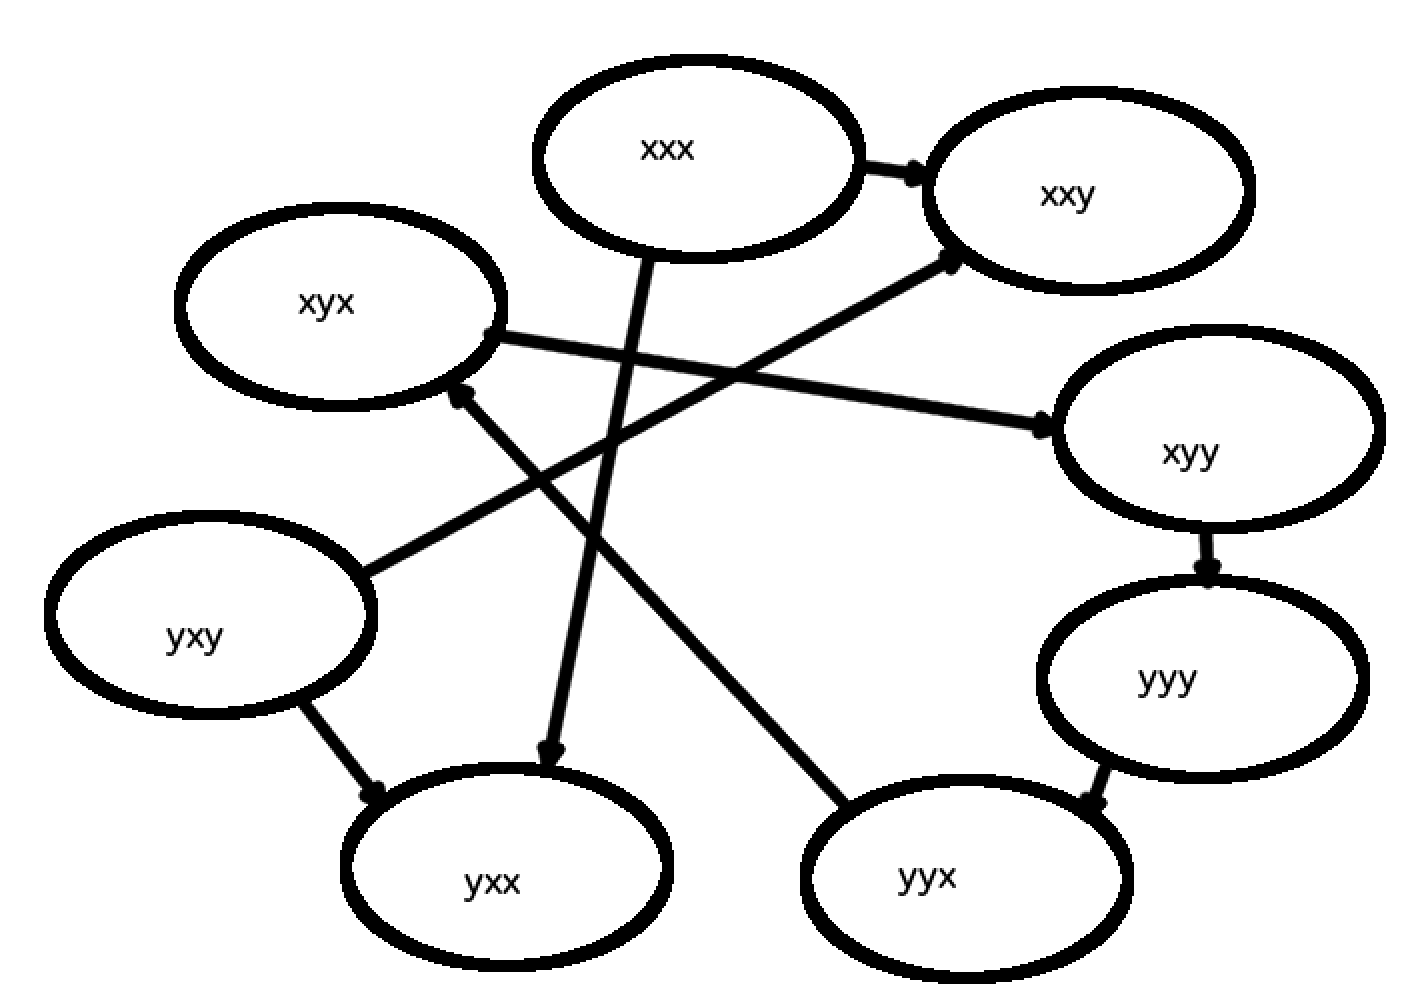
\includegraphics[width=10cm]{f2}
  \end{center}
  \end{figure}

  \item{What are the N.E.?}\\
    $yxx$ and $xyy$ are the NE.

  \item{How does the price of anarchy of this game compare to the setting in Part \#1?}
    This game's BRG has a cycle, meaning that there is a situation where no Nash equilibrium
    is reached.  Since this is not an equilibrium, however, it has no bearing on the PoA.  Both
    games have the same N.E. and the same utilitarian cost function, they must also have the same
    PoA.

\end{enumerate}

\textbf{2)} Consider the following two player game with the (utility) payoff matrix:

\begin{center}
  \begin{tabular}{r |c|c|}
    \multicolumn{1}{r}{}
    & \multicolumn{1}{c}{$a_2$}
    & \multicolumn{1}{c}{$b_2$}\\
    \cline{2-3}
    $a_1$ & 3,3 & 0,4 \\
    \cline{2-3}
    $b_1$ & 4,0 & 1,1 \\
    \cline{2-3}
  \end{tabular}
\end{center}
\begin{enumerate}[(a)]
  \item{What are the analytical stationary distrobutions when $T=0.1, 1, 10,$ and $100$ for
    log-linear learning?}\\
    This is a potential game with potential function $\Phi$:
\begin{center}
  \begin{tabular}{r |c|c|}
    \multicolumn{1}{r}{}
    & \multicolumn{1}{c}{$a_2$}
    & \multicolumn{1}{c}{$b_2$}\\
    \cline{2-3}
    $a_1$ & 0 & 1 \\
    \cline{2-3}
    $b_1$ & 1 & 2 \\
    \cline{2-3}
  \end{tabular}
\end{center}
We know that for a potential game like this, finding the stationary distrobution is quite easy,
for $T=0.1$:
\begin{center}
  \begin{tabular}{r |c|c|}
    \multicolumn{1}{r}{}
    & \multicolumn{1}{c}{$a_2$}
    & \multicolumn{1}{c}{$b_2$}\\
    \cline{2-3}
    $a_1$ & 0.0000 & 0.0000 \\
    \cline{2-3}
    $b_1$ & 0.0000 & 0.9999 \\
    \cline{2-3}
  \end{tabular}
\end{center}

for $T=1$:

\begin{center}
  \begin{tabular}{r |c|c|}
    \multicolumn{1}{r}{}
    & \multicolumn{1}{c}{$a_2$}
    & \multicolumn{1}{c}{$b_2$}\\
    \cline{2-3}
    $a_1$ & 0.0723 & 0.1966 \\
    \cline{2-3}
    $b_1$ & 0.1966 & 0.5344 \\
    \cline{2-3}
  \end{tabular}
\end{center}

for $T=10$:

\begin{center}
  \begin{tabular}{r |c|c|}
    \multicolumn{1}{r}{}
    & \multicolumn{1}{c}{$a_2$}
    & \multicolumn{1}{c}{$b_2$}\\
    \cline{2-3}
    $a_1$ & 0.2256 & 0.2494 \\
    \cline{2-3}
    $b_1$ & 0.2494 & 0.2756 \\
    \cline{2-3}
  \end{tabular}
\end{center}

for $T=100$:

\begin{center}
  \begin{tabular}{r |c|c|}
    \multicolumn{1}{r}{}
    & \multicolumn{1}{c}{$a_2$}
    & \multicolumn{1}{c}{$b_2$}\\
    \cline{2-3}
    $a_1$ & 0.2475 & 0.2500 \\
    \cline{2-3}
    $b_1$ & 0.2500 & 0.2525 \\
    \cline{2-3}
  \end{tabular}
\end{center}

\item{Write a Matlab script to simulate the above game using Log-Linear Learning.  Verify
  that the empirical distrobution approaches your analytical predictions for the previous
  problem.(plot empirical distrobution vs. iteration for each of the four joint action)}

  The matlab script shows us the empirical distrobution vs. iteration for each joint action as
  $T\rightarrow0$:

  \begin{figure}[H]
  \begin{center}
  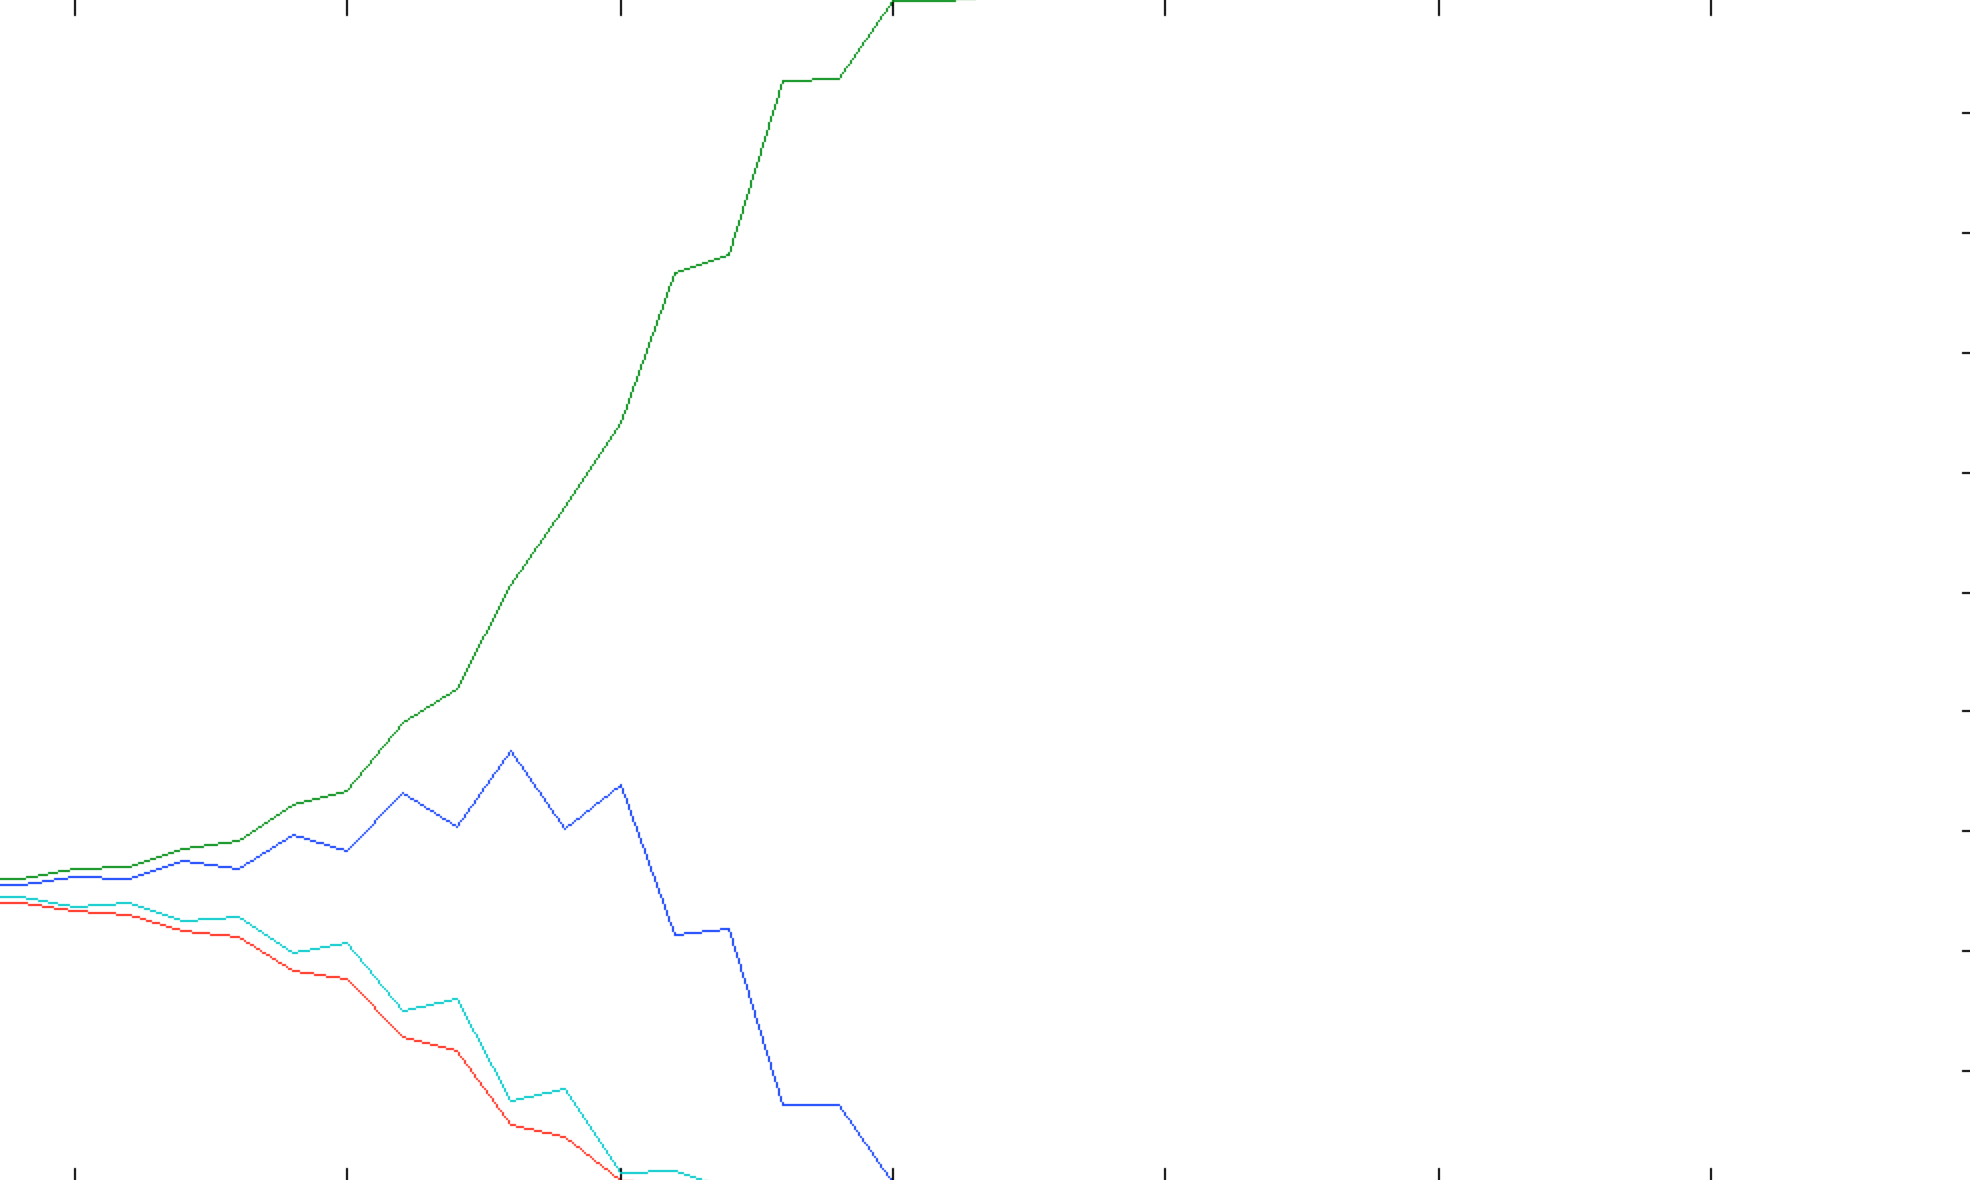
\includegraphics[width=10cm]{f3}
  \end{center}
  \end{figure}

  the green line is $b_1b_2$, the eventual joint distrobution.
\end{enumerate}

\textbf{3)} Write a Matlab script to solve $4\times4$ Sudoku using Log-Linear Learning.
If you haven't already, Insert a "kick out" test that terminates the iterations upon
solution of the puzzle.

\end{document}
